% Provenance (never printed): old premiere S material on plate kinematics (rigid
% plates, rates from magnetic anomalies and from satellite positioning, hotspots
% and the Hawaiian chain, the coherence of the model); see
% sources/book2/PROVENANCE.md. Velocities from the NNR-MORVEL56 poles
% (figdata/grade-11/plate_velocities.py), station series from the Nevada Geodetic
% Laboratory (gnss_series.py), volcano ages from Clague and Dalrymple 1987
% (hawaii_chain.py). Euler poles and triple junctions belong to Year 1: the
% rotation pole is told, not defined.
\chapter{Les plaques et leurs mouvements}\label{ch:g11:plate-motions}

Près du sommet du Mauna Kea, sur l'île d'Hawaï, une antenne fixée à la
roche reçoit chaque jour depuis octobre 1996 les signaux des satellites de
positionnement. Chaque jour, un ordinateur calcule la position de l'antenne,
à quelques millimètres près. Trente ans de positions racontent la même
histoire année après année~: l'antenne, la montagne et l'île tout entière se
déplacent d'environ \qty{7}{cm} par an vers l'ouest-nord-ouest, sans
s'arrêter et sans tourner. En 2026, l'antenne se trouvait à plus de deux
mètres de son point de départ. Ce chapitre mesure de tels mouvements, montre
comment ils s'accordent sur une sphère, et lit le même mouvement dans la
chaîne de volcans éteints qui s'étire depuis Hawaï à travers le Pacifique
Nord.
% ledger: data:b2-ngl-gnss

\begin{recall}
La \omterm{def:g11:lithosphere-asthenosphere:lithosphere}{lithosphère} est découpée en plaques tectoniques qui se déplacent les unes
par rapport aux autres de quelques centimètres par an~; leurs limites sont
des dorsales, des fosses, des zones de collision et des failles
transformantes (livre~1, année~7). Un point chaud est un endroit situé en
profondeur dans le manteau qui alimente un volcan sur la plaque qui le
surmonte~; la plaque emporte le volcan tandis qu'un nouveau volcan se forme
au-dessus du point chaud (livre~1, année~7). Un récepteur de positionnement
par satellite calcule sa propre position à partir des signaux de plusieurs
satellites (livre~1, année~9). Les bandes magnétiques du fond océanique
donnent la \omterm{def:g11:drift-to-spreading:spreading-rate}{vitesse d'expansion} d'une dorsale
(\cref{ch:g11:drift-to-spreading}), et la \omterm{def:g11:lithosphere-asthenosphere:lithosphere}{lithosphère} est l'enveloppe
externe rigide de la Terre, épaisse d'environ \qty{100}{km}
(\cref{ch:g11:lithosphere-asthenosphere}). Une vitesse de \qty{1}{cm} par an
correspond à \qty{10}{km} par million d'années, et \qty{1}{mm} par an à
\qty{1}{km} par million d'années.
\end{recall}

\begin{omfigure}
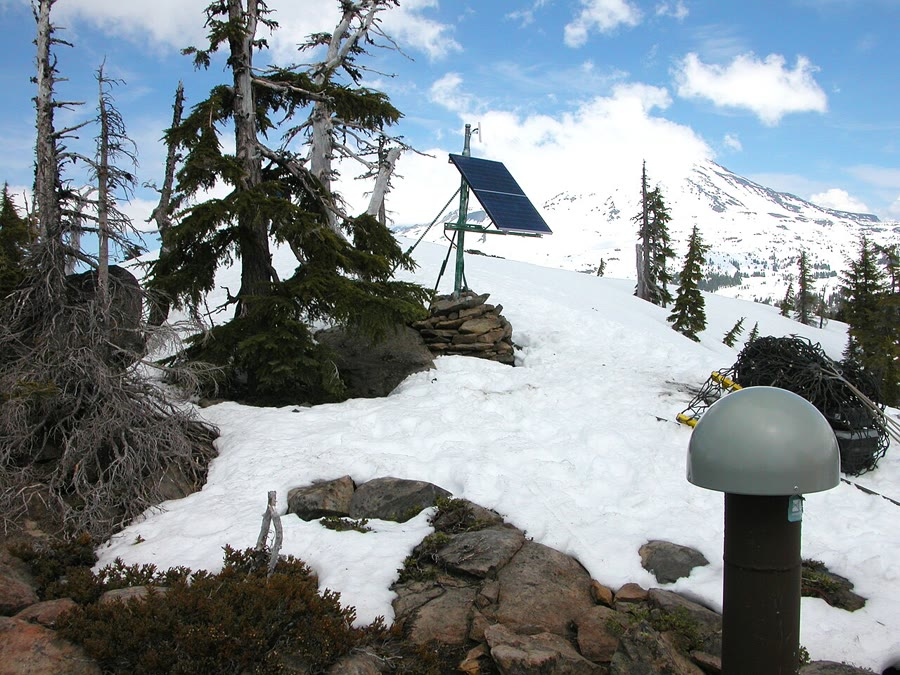
\includegraphics[width=0.62\linewidth]{images/book2/g11-usgs-gps-station.jpg}

{\small Une station permanente de positionnement par satellite sur un volcan
de la chaîne des Cascades, en Oregon (2007). L'antenne se trouve sous le
dôme gris, sur un mât solidement ancré dans le sol~; le panneau solaire
situé derrière alimente le récepteur. Une telle station enregistre sa propre
position jour après jour. Photographie~: Dave Sherrod, USGS (domaine
public).}
\end{omfigure}
% ledger: photo:g11-gps-station

\section{Des plaques rigides sur une sphère}

Les séismes ne sont pas dispersés au hasard sur la Terre~: presque tous se
produisent le long de ceintures étroites, les limites de plaques (livre~1,
année~7). À l'intérieur d'une plaque, la roche ne se rompt presque jamais.
Une plaque n'est donc pas une peau souple qui s'étire et se plisse en se
déplaçant, mais un morceau rigide de \omterm{def:g11:lithosphere-asthenosphere:lithosphere}{lithosphère} qui se déplace d'un seul
tenant.

\begin{definition}[Plaque rigide]\label{def:g11:plate-motions:rigid-plate}
Une \emph{plaque rigide}\index{plaque rigide} est un morceau de \omterm{def:g11:lithosphere-asthenosphere:lithosphere}{lithosphère}
qui se déplace d'un seul bloc~: les distances entre ses points ne changent
pas, et sa déformation est concentrée dans des zones étroites le long de ses
limites.
\end{definition}

Le modèle des \omterm{def:g11:plate-motions:rigid-plate}{plaques rigides} est une approximation. Certaines régions se
déforment sur des centaines de kilomètres, comme les hauts plateaux situés
derrière l'Himalaya ou l'ouest de l'Amérique du Nord, et le modèle les
traite comme des limites larges. Mais sur la plus grande partie de la
surface de la Terre, il fonctionne remarquablement bien~: les vitesses qu'il
prévoit pour des \omterm{def:g11:plate-motions:rigid-plate}{plaques rigides} concordent à quelques millimètres par an
près avec celles que mesurent les stations satellitaires
(\cref{sec:g11:plate-motions:predictive}), alors que les plaques se
déplacent les unes par rapport aux autres de plusieurs centimètres par an.

Comment une calotte rigide peut-elle se déplacer à la surface d'une
sphère~? Elle ne peut pas glisser en ligne droite, car une ligne droite
quitte la sphère. Quel que soit le mouvement d'une calotte rigide, c'est une
\emph{rotation} autour d'un axe passant par le centre de la Terre. L'axe
perce la surface au \emph{pôle de rotation} de la plaque. Un point de la
plaque se déplace le long d'un petit cercle autour de ce pôle, et plus il
est loin du pôle, plus son cercle est grand et plus il va vite (figure
ci-dessous). La démonstration que tout mouvement d'une calotte rigide est
une telle rotation, et l'usage des pôles de rotation pour décrire les
limites de plaques, relèvent du livre~3~; on n'utilise ici que les vitesses.

\begin{omfigure}
\begin{tikzpicture}[scale=1.15, font=\footnotesize]
  \fill[omSea!45] (0,0) circle (2);
  \draw (0,0) circle (2);
  % small circles about the rotation pole (pole at the top), seen slightly from above
  \foreach \a/\len in {60/0.75, 35/1.23, 0/1.5} {
    \pgfmathsetmacro{\r}{2*cos(\a)}
    \pgfmathsetmacro{\h}{2*sin(\a)}
    \draw[black!45, densely dashed] (-\r,\h) arc[start angle=180, end angle=0, x radius=\r, y radius=0.22*\r];
    \draw[omDef!80!black, line width=0.7pt] (-\r,\h) arc[start angle=180, end angle=360, x radius=\r, y radius=0.22*\r];
    \draw[-{Stealth[length=5pt]}, omProp, line width=1.1pt] (0,\h-0.22*\r) -- ++(\len,0);
  }
  \draw[black!70, dash pattern=on 3pt off 2pt] (0,-2.5) -- (0,2.55);
  \fill (0,2) circle (1.6pt);
  \node[anchor=south west] at (0.05,2.02) {pôle de rotation};
  \node[anchor=north, text=black!70] at (0,-2.5) {axe de rotation, passant par le centre};
  \fill (0,0) circle (1pt);
  \node[anchor=west, align=left] at (2.25,0.9) {chaque point se déplace\\le long d'un petit cercle\\autour du pôle};
  \node[anchor=west, align=left, text=omProp] at (2.25,-0.4) {vitesse maximale\\à \ang{90} du pôle};
\end{tikzpicture}

{\small Une \omterm{def:g11:plate-motions:rigid-plate}{plaque rigide} sur une sphère tourne autour d'un axe passant par
le centre de la Terre. Les points proches du pôle de rotation se déplacent
lentement, le long de petits cercles~; les points situés à \ang{90} du pôle
se déplacent le plus vite (flèches~: vitesses à l'échelle).}
\end{omfigure}

La vitesse d'un point se calcule facilement. Un point situé à la distance
angulaire $\theta$ du pôle se trouve à la distance $R\sin\theta$ de l'axe,
où $R = \qty{6371}{km}$ est le rayon de la Terre. Si la plaque tourne de
$\omega$ degrés par million d'années, le point parcourt en un million
d'années la fraction $\omega/360$ du cercle de rayon $R\sin\theta$~:
\[
  v = \frac{\omega}{360} \times 2\pi R\sin\theta
    = \frac{\pi\,\omega}{180}\,R\sin\theta .
\]
Pour $\omega = \qty{1}{\degree}$ par million d'années et $\theta = \ang{90}$,
cela donne $\pi \times 6371/180 \approx \qty{111}{km}$ par million d'années,
soit \qty{11.1}{cm} par an. Une plaque n'a donc pas une vitesse unique~: ses
points se déplacent à des vitesses qui vont de zéro au pôle de rotation (si
le pôle se trouve sur la plaque) à un maximum à \ang{90} de celui-ci. Les
failles transformantes d'une dorsale, qui permettent à deux plaques de
coulisser l'une contre l'autre, suivent des petits cercles autour du pôle de
la rotation relative des deux plaques.
% ledger: earth:Rmean (shared), nnr56:poles

Des jeux de pôles de rotation publiés donnent, pour chaque plaque, la
position de son pôle et sa vitesse de rotation. L'un d'eux, construit
surtout à partir des vitesses et des directions d'expansion mesurées le long
des dorsales, décrit 56 plaques~; la plaque Pacifique tourne de
\ang{0.651} par million d'années, la plaque eurasiatique de \ang{0.223}. À
partir de ces nombres, un ordinateur calcule la vitesse de n'importe quel
point de n'importe quelle plaque (carte ci-dessous).
% ledger: nnr56:poles, nnr56:data

\begin{omfigure}
\begin{tikzpicture}
\begin{axis}[ommap, width=\linewidth, xtick={-180,-90,...,180}, ytick={-60,0,60}]
\addplot[fill=omLithAlluv, draw=black!45, line width=0.2pt] table {figdata/out/shared-geo-land.dat};
\addplot[omRidge, line width=0.6pt] table {figdata/out/shared-geo-school-ridge.dat};
\addplot[omRidge!70!black, line width=0.6pt] table {figdata/out/shared-geo-school-transform.dat};
\addplot[omTrench, line width=0.6pt] table {figdata/out/shared-geo-school-subduction.dat};
\addplot[fill=omTrench, draw=none] table {figdata/out/shared-geo-school-teeth.dat};
\addplot[black!65, line width=0.6pt] table {figdata/out/shared-geo-school-collision.dat};
% computed in figdata/grade-11/plate_velocities.py (NNR-MORVEL56); 2.5 degrees per cm/yr
\addplot[black, line width=0.8pt, -{Stealth[length=4pt]}, quiver={u=\thisrow{dx}, v=\thisrow{dy}}]
  table[x=lon, y=lat] {figdata/out/grade-11-plate_velocities-arrows.dat};
\addplot[omProp, line width=1.2pt, -{Stealth[length=5pt]}, quiver={u=\thisrow{dx}, v=\thisrow{dy}}]
  table[x=lon, y=lat] {figdata/out/grade-11-plate_velocities-hawaii.dat};
\addplot[only marks, mark=*, mark size=1.3pt, omProp] coordinates {(-155.46,19.80)};
\node[font=\scriptsize, anchor=north, fill=white, fill opacity=0.75, text opacity=1, inner sep=1pt]
  at (axis cs:-150,15) {Mauna Kea};
\draw[black, line width=0.8pt, -{Stealth[length=4pt]}] (axis cs:-172,-80) -- (axis cs:-147,-80);
\node[font=\scriptsize, anchor=west, fill=white, fill opacity=0.75, text opacity=1, inner sep=1pt]
  at (axis cs:-145,-80) {\qty{10}{cm} par an};
\end{axis}
\end{tikzpicture}

{\small Les vitesses de points situés à l'intérieur de 16 plaques,
calculées à partir de leurs pôles de rotation publiés, dans un référentiel
dans lequel la \omterm{def:g11:lithosphere-asthenosphere:lithosphere}{lithosphère} dans son ensemble ne tourne pas. Les plaques
Pacifique, de Nazca, des Cocos, australienne et indienne se déplacent le
plus vite~; les plaques eurasiatique, nord-américaine, sud-américaine et
antarctique lentement. Flèche rouge~: la plaque Pacifique au Mauna Kea.
Pôles de rotation~: Argus, Gordon et DeMets (2011)~; limites de plaques~:
Bird (2003)~; terres émergées~: Natural Earth.}
\end{omfigure}
% ledger: nnr56:poles, data:pb2002, data:ne-land

\section{Mesurer les mouvements}

\subsection{Deux façons de mesurer une vitesse}

Les bandes magnétiques du fond océanique donnent la vitesse à laquelle deux
plaques s'écartent de part et d'autre d'une dorsale
(\cref{ch:g11:drift-to-spreading})~: on divise la distance d'une bande à
l'axe de la dorsale par son âge. La vitesse obtenue est une moyenne sur
l'âge de la bande, souvent les derniers millions d'années, et c'est une
vitesse \emph{relative}, celle d'une plaque vue depuis l'autre. Les bandes
ne disent rien des plaques qui se rencontrent à une fosse ou dans une zone
de collision, puisqu'il ne s'y forme pas de fond océanique.

Le positionnement par satellite mesure le mouvement d'un point unique,
aujourd'hui, sur quelques années ou décennies. Une station permanente est
ancrée dans la roche en place, de sorte qu'elle se déplace avec la
plaque~; ses positions quotidiennes, reportées en fonction du temps,
s'alignent sur une droite dont la pente est la vitesse de la station.

\begin{method}[Une vitesse d'après une série temporelle de positions]\label{met:g11:plate-motions:rate}
\begin{enumerate}
  \item Reporter la position est et la position nord de la station en
        fonction du temps, sur deux graphiques ou sur le même.
  \item Tracer la droite qui suit le mieux chaque série (ou y lire deux
        points éloignés). Sa pente, en millimètres par an, est la vitesse
        vers l'est $v_E$ ou la vitesse vers le nord $v_N$~; une station qui
        se déplace vers l'ouest ou vers le sud a une vitesse négative.
  \item La vitesse de la station vaut $v = \sqrt{v_E^2 + v_N^2}$~; sa
        direction fait avec la ligne est--ouest l'angle $\alpha$ tel que
        $\tan\alpha = |v_N|/|v_E|$, vers le nord si $v_N > 0$ et vers
        l'est si $v_E > 0$.
\end{enumerate}
\end{method}

\begin{omfigure}
\begin{tikzpicture}
\begin{axis}[ompt, name=a, width=0.5\linewidth, height=5.6cm, xmin=1995, xmax=2027, ymin=-200, ymax=120,
  xlabel={année}, ylabel={position (\unit{cm})}, xtick={2000,2010,2020},
  xticklabel style={/pgf/number format/set thousands separator={}},
  title={\small Mauna Kea, Hawaï (MKEA)}, tick label style={font=\scriptsize}]
% computed in figdata/grade-11/gnss_series.py; ledger: data:b2-ngl-gnss
\addplot[only marks, mark=*, mark size=0.5pt, omDef] table[x=year, y=north] {figdata/out/grade-11-gnss_series-mkea.dat};
\addplot[only marks, mark=*, mark size=0.5pt, omProp] table[x=year, y=east] {figdata/out/grade-11-gnss_series-mkea.dat};
\node[font=\scriptsize, text=omDef!80!black, anchor=west] at (axis cs:1996.5,80) {nord};
\node[font=\scriptsize, text=omProp!80!black, anchor=west] at (axis cs:1996.5,-120) {est};
\end{axis}
\begin{axis}[ompt, at={(a.east)}, anchor=west, xshift=0.9cm, width=0.5\linewidth, height=5.6cm, xmin=1995, xmax=2027,
  ymin=-10, ymax=70, xlabel={année}, xtick={2000,2010,2020},
  xticklabel style={/pgf/number format/set thousands separator={}},
  title={\small Wettzell, Allemagne (WTZR)}, tick label style={font=\scriptsize}]
\addplot[only marks, mark=*, mark size=0.5pt, omDef] table[x=year, y=north] {figdata/out/grade-11-gnss_series-wtzr.dat};
\addplot[only marks, mark=*, mark size=0.5pt, omProp] table[x=year, y=east] {figdata/out/grade-11-gnss_series-wtzr.dat};
\node[font=\scriptsize, text=omDef!80!black, anchor=west] at (axis cs:2014,22) {nord};
\node[font=\scriptsize, text=omProp!80!black, anchor=west] at (axis cs:2006,40) {est};
\end{axis}
\end{tikzpicture}

{\small Positions moyennes mensuelles de deux stations permanentes, mesurées
à partir de leur premier mois~: est (en rouge) et nord (en bleu). Chaque
série s'aligne sur une droite, dont la pente est la vitesse de la station
dans cette direction. Le Mauna Kea, sur la plaque Pacifique, se déplace vers
l'ouest et vers le nord~; Wettzell, sur la plaque eurasiatique, vers l'est
et vers le nord, environ trois fois plus lentement. Données~: Nevada
Geodetic Laboratory (Blewitt, Hammond et Kreemer, 2018).}
\end{omfigure}
% ledger: data:b2-ngl-gnss

\begin{example}[La station du Mauna Kea]\label{ex:g11:plate-motions:mkea}
D'octobre 1996 à septembre 2026, les positions mensuelles de la station du
Mauna Kea suivent deux droites de pentes $v_E =
\qty{-63.2}{mm}$ par an (vers l'ouest) et $v_N = \qty{+34.5}{mm}$ par an. La
vitesse vaut $\sqrt{63.2^2 + 34.5^2} \approx \qty{72}{mm}$ par an, et $\tan\alpha
= 34.5/63.2 \approx 0.546$ donne $\alpha \approx \ang{29}$~: la station se
déplace de \qty{7.2}{cm} par an dans une direction située à \ang{29} au nord
de l'ouest. Le pôle de rotation de la plaque Pacifique prévoit, en ce lieu,
\qty{6.9}{cm} par an, à \ang{28} au nord de l'ouest.
\end{example}
% ledger: data:b2-ngl-gnss, nnr56:poles (prediction computed in plate_velocities.py)

Les points s'écartent de quelques millimètres de part et d'autre des
droites, bien moins que le mouvement d'une seule année~: après quelques
années de mesure, la vitesse d'une station est connue à mieux d'un
millimètre par an près.

\subsection{Mouvement relatif et mouvement absolu}

Une vitesse se mesure toujours par rapport à quelque chose. La station du
Mauna Kea se déplace de \qty{7.2}{cm} par an par rapport à un référentiel
lié à la Terre entière~; vue depuis une station d'Amérique du Nord, qui se
déplace elle-même, sa vitesse est différente.

\begin{definition}[Mouvement relatif~; mouvement absolu]\label{def:g11:plate-motions:relative-motion}
Le \emph{mouvement relatif}\index{mouvement relatif} d'une plaque $A$ par
rapport à une plaque $B$ est son mouvement tel que le voit un observateur
placé sur $B$. Le \emph{mouvement absolu}\index{mouvement absolu} d'une
plaque est son mouvement par rapport à un référentiel lié à la Terre
profonde, par exemple un ensemble de points chauds supposés fixes, ou le
référentiel dans lequel la \omterm{def:g11:lithosphere-asthenosphere:lithosphere}{lithosphère} dans son ensemble ne tourne pas.
\end{definition}

Les dorsales, les fosses et les failles transformantes sont façonnées par
les \omterm{def:g11:plate-motions:relative-motion}{mouvements relatifs}~: ce qui compte à une limite, c'est la façon dont
les deux plaques se déplacent l'une par rapport à l'autre. Les vitesses
relatives s'additionnent comme les déplacements qu'elles produisent.

\begin{proposition}[Les vitesses relatives s'additionnent comme des flèches]\label{prop:g11:plate-motions:sum}
Soit $\vec v_{A/B}$ la vitesse de la plaque $A$ par rapport à la plaque $B$,
en un point donné de la limite, et de même pour les autres paires. Pour
trois plaques quelconques $A$, $B$, $C$,
\[
  \vec v_{A/C} = \vec v_{A/B} + \vec v_{B/C},
  \qquad\text{et}\qquad
  \vec v_{B/A} = -\vec v_{A/B}.
\]
\end{proposition}

\begin{proof}
Pendant une courte durée $\Delta t$, soit un point lié à $A$ qui passe de la
position $P$ à $P'$ vu depuis $C$, et soit le point de $B$ qui était en $P$
et qui passe en $Q$ vu depuis $C$. Vu depuis $B$, le point de $A$ est passé
de $Q$ à $P'$. Les déplacements s'additionnent comme des vecteurs~:
$\overrightarrow{PP'} = \overrightarrow{PQ} + \overrightarrow{QP'}$,
c'est-à-dire~: déplacement de $A$ vu depuis $C$ = déplacement de $B$ vu
depuis $C$ + déplacement de $A$ vu depuis $B$. En divisant par $\Delta t$,
on obtient $\vec v_{A/C}
= \vec v_{B/C} + \vec v_{A/B}$. Avec $C = A$, le membre de gauche est
nul~: $\vec
v_{B/A} = -\vec v_{A/B}$.
\end{proof}

\begin{method}[Fermer un triangle des vitesses]\label{met:g11:plate-motions:triangle}
\begin{enumerate}
  \item Écrire chaque vitesse connue avec ses composantes est et nord,
        toutes mesurées au même point.
  \item Pour trouver $\vec v_{A/B}$ à partir des vitesses de $A$ et de $B$
        dans le même référentiel $C$, soustraire~: $\vec v_{A/B} = \vec v_{A/C} - \vec v_{B/C}$,
        composante par composante.
  \item Sur un dessin, placer l'origine de $\vec v_{A/C}$ et celle de
        $\vec v_{B/C}$ au même point~: la flèche qui va de la pointe de
        $\vec v_{B/C}$ à la pointe de $\vec v_{A/C}$ est $\vec v_{A/B}$, et
        elle ferme le triangle.
  \item Calculer sa longueur et sa direction comme dans la
        \cref{met:g11:plate-motions:rate}.
\end{enumerate}
\end{method}

\begin{example}[La faille de San Andreas]\label{ex:g11:plate-motions:san-andreas}
En Californie centrale, à \ang{35.5} Nord et \ang{120.5} Ouest, les pôles de
rotation donnent à la plaque Pacifique la vitesse $(-42.1, +26.4)$ et à la
plaque nord-américaine $(-11.9, -14.8)$, en millimètres par an (est, nord),
dans le référentiel de l'ensemble de la \omterm{def:g11:lithosphere-asthenosphere:lithosphere}{lithosphère}. La plaque Pacifique se
déplace par rapport à l'Amérique du Nord à $(-42.1 + 11.9,\ 26.4 + 14.8) = (-30.2, +41.2)$, soit
$\sqrt{30.2^2 + 41.2^2} \approx \qty{51}{mm}$ par an, dans une direction
située à \ang{36} à l'ouest du nord (figure ci-dessous). La faille de San
Andreas, orientée nord-ouest, absorbe la plus grande partie de ce
coulissement.
\end{example}
% ledger: nnr56:poles (computed in plate_velocities.py: relative pa/na at 120.5 W 35.5 N)

\begin{omfigure}
\begin{tikzpicture}[x=0.065cm, y=0.065cm, font=\footnotesize]
  % mm/yr, from plate_velocities.py: PA (-42.1, 26.4), NA (-11.9, -14.8), PA/NA (-30.2, 41.2)
  \draw[black!25] (-8,0) -- (8,0) (0,-8) -- (0,8);
  \draw[-{Stealth[length=5pt]}, omProp, line width=1.1pt] (0,0) -- (-42.1,26.4)
    node[pos=0.55, above right, inner sep=1pt] {$\vec v_{\mathrm{PA}}$};
  \draw[-{Stealth[length=5pt]}, omDef, line width=1.1pt] (0,0) -- (-11.9,-14.8)
    node[pos=0.8, right=2pt] {$\vec v_{\mathrm{NA}}$};
  \draw[-{Stealth[length=5pt]}, black, line width=1.1pt] (-11.9,-14.8) -- (-42.1,26.4)
    node[pos=0.4, left=9pt, align=right] {$\vec v_{\mathrm{PA/NA}}$\\\qty{51}{mm} par an};
  \fill (0,0) circle (0.9pt);
  % compass
  \draw[-{Stealth[length=4pt]}] (25,10) -- (25,24) node[above] {N};
  \draw[-{Stealth[length=4pt]}] (25,10) -- (39,10) node[right] {E};
  \draw (25,-18) -- (40.4,-18);
  \node[below] at (32.7,-18) {\qty{20}{mm} par an};
  \draw (25,-17) -- (25,-19) (40.4,-17) -- (40.4,-19);
\end{tikzpicture}

{\small Fermeture d'un triangle des vitesses en Californie centrale (à
l'échelle). En rouge~: la plaque Pacifique~; en bleu~: la plaque
nord-américaine, toutes deux dans le référentiel de l'ensemble de la
\omterm{def:g11:lithosphere-asthenosphere:lithosphere}{lithosphère}. En noir~: la plaque Pacifique vue depuis l'Amérique du Nord,
la flèche qui va de la pointe de la bleue à la pointe de la rouge.}
\end{omfigure}

\section{Les traces de points chauds}

\subsection{Une plaque au-dessus d'un panache fixe}

Hawaï se trouve au milieu de la plaque Pacifique, à plus de \qty{3000}{km}
de la limite de plaques la plus proche.
% ledger: usgs:hawaii-hotspot (Book 1 row)
 Ses volcans sont alimentés par un point chaud (livre~1,
année~7). La plaque se déplace au-dessus de lui, et chaque volcan est
emporté loin du point chaud tandis qu'un nouveau se forme derrière lui.

\begin{definition}[Trace de point chaud]\label{def:g11:plate-motions:hotspot-track}
Une \emph{trace de point chaud}\index{trace de point chaud} est l'alignement
de volcans, et des volcans engloutis appelés monts sous-marins, qu'une
plaque emporte loin d'un point chaud en se déplaçant au-dessus de lui~: le
volcan actif se trouve au-dessus du point chaud, et les volcans sont de plus
en plus anciens à mesure qu'on s'en éloigne.
\end{definition}

\begin{omfigure}
\begin{tikzpicture}[font=\footnotesize]
  % plate moving to the left over a fixed plume (not to scale)
  \fill[omSea!50] (0,0) rectangle (11,0.9);
  \fill[black!22] (0,-0.9) rectangle (11,0);
  \draw (0,0) -- (11,0);
  \draw[densely dashed] (0,0.9) -- (11,0.9) node[right] {niveau de la mer};
  \node[anchor=east] at (10.95,-0.45) {lithosphère};
  \fill[omLithPeridotite!40] (0,-2.3) rectangle (11,-0.9);
  \node[anchor=west] at (0.1,-1.6) {asthénosphère};
  % plume
  \fill[omProp!55] (8.6,-2.3) -- (8.6,-1.2) .. controls (8.6,-0.9) and (9.2,-0.9) .. (9.2,-1.2) -- (9.2,-2.3) -- cycle;
  \fill[omProp!55] (8.75,-0.95) rectangle (9.05,0);
  \node[anchor=north, align=center] at (8.9,-2.35) {panache, fixe dans le manteau};
  % volcanoes: active over the plume, older ones carried left, eroded and sunk
  \fill[black!65] (8.0,0) -- (8.9,1.6) -- (9.8,0) -- cycle;
  \fill[black!55] (5.4,0) -- (6.2,1.15) -- (7.0,0) -- cycle;
  \fill[black!50] (3.0,0) -- (3.55,0.62) -- (3.85,0.62) -- (4.4,0) -- cycle;
  \fill[black!45] (0.8,0) -- (1.25,0.42) -- (1.65,0.42) -- (2.1,0) -- cycle;
  \node[above] at (8.9,1.6) {actif};
  \node[above] at (6.2,1.15) {$t_1$};
  \node[above] at (3.7,0.62) {$t_2$};
  \node[above] at (1.45,0.42) {$t_3$};
  % plate motion
  \draw[-{Stealth[length=6pt]}, line width=1.2pt] (6.5,-0.45) -- (4.0,-0.45) node[left] {la plaque avance, vitesse $v$};
  % distance d = v t
  \draw[{Stealth[length=4pt]}-{Stealth[length=4pt]}] (3.7,2.3) -- (8.9,2.3) node[midway, above] {$d_2 = v\,t_2$};
  \draw[black!50] (3.7,1.05) -- (3.7,2.4) (8.9,2.0) -- (8.9,2.4);
\end{tikzpicture}

{\small Une plaque qui se déplace à la vitesse $v$ au-dessus d'un panache
fixe dans le manteau (sans échelle). Un volcan d'âge $t$, construit
au-dessus du panache, a été emporté sur la distance $d = v\,t$~; les volcans
plus anciens sont érodés et s'enfoncent sous la mer.}
\end{omfigure}

\begin{proposition}[Vitesse d'après une trace de point chaud]\label{prop:g11:plate-motions:hotspot}
Si un point chaud reste fixe dans le manteau profond et si la plaque qui le
surmonte se déplace à une vitesse $v$ constante dans une direction
constante, un volcan qui se trouvait au-dessus du point chaud il y a un
temps $t$ se trouve maintenant à la distance
\[
  d = v\,t
\]
du volcan actif, le long de la trace. Les âges des volcans, reportés en
fonction de leurs distances, s'alignent sur une droite passant par l'origine
dont la pente vaut $1/v$, et $v$ est la vitesse absolue de la plaque.
\end{proposition}

\begin{proof}
Le volcan s'est construit là où la plaque se trouvait au-dessus du point
chaud, et il s'est déplacé avec la plaque depuis. Pendant la durée $t$, la
plaque s'est déplacée de $v\,t$ dans une direction fixe~: le volcan se
trouve donc à cette distance du point de la plaque situé maintenant
au-dessus du point chaud, là où se dresse le volcan actif. La relation
$t = d/v$ est celle d'une droite passant par l'origine, de pente $1/v$. La
vitesse est mesurée par rapport au point chaud, c'est-à-dire par rapport au
manteau profond~: c'est une vitesse absolue.
\end{proof}

\subsection{La chaîne Hawaï--Empereur}

Depuis l'île d'Hawaï, un alignement d'îles, de récifs et de monts
sous-marins s'étend sur quelque \qty{3400}{km} vers l'ouest-nord-ouest, puis
tourne brusquement et se poursuit vers le nord sous le nom de monts
sous-marins de l'Empereur, le seul mont sous-marin Suiko se trouvant à
\qty{4860}{km} de Kilauea, jusqu'aux fosses qui longent le Kamtchatka et
les Aléoutiennes (image ci-dessous).
% ledger: cd87:ages

\begin{omfigure}
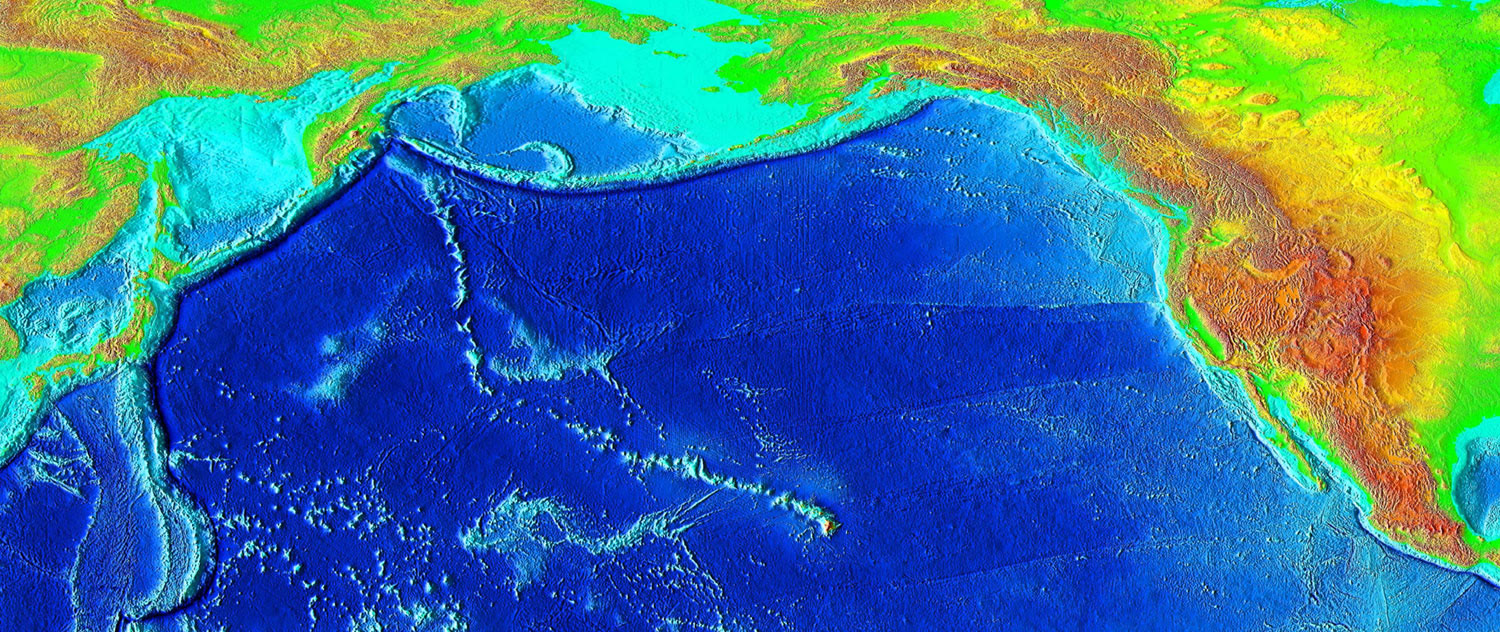
\includegraphics[width=\linewidth]{images/book2/g11-ngdc-hawaii-chain.jpg}

{\small Relief ombré du fond du Pacifique Nord. La chaîne hawaïenne part de
l'île d'Hawaï (en bas au centre, en brun) vers l'ouest-nord-ouest~; au
coude, elle tourne vers le nord pour former les monts sous-marins de
l'Empereur, qui s'achèvent à la fosse qui longe le Kamtchatka et les
Aléoutiennes. Image~: National Geophysical Data Center, NOAA (domaine
public).}
\end{omfigure}
% ledger: photo:g11-hawaii-chain

La datation potassium--argon de laves de 37 volcans de la chaîne, récoltées
sur les îles, draguées sur les monts sous-marins ou prélevées par forage à
travers leurs sédiments, donne leurs âges (graphique ci-dessous). Le Mauna
Kea a environ \num{0.4} million d'années, Kauai \num{5.1}, Midway
\num{27.7}, et le mont sous-marin Suiko, près de l'extrémité de la chaîne de
l'Empereur, \num{64.7}. Les âges augmentent avec la distance à Kilauea, le
volcan actif, comme le prévoit une \omterm{def:g11:plate-motions:hotspot-track}{trace de point chaud}.
% ledger: cd87:ages

\begin{omfigure}
\begin{tikzpicture}
\begin{axis}[ompt, width=0.82\linewidth, height=6.4cm, xmin=0, xmax=5000, ymin=0, ymax=70,
  xlabel={distance à Kilauea le long de la chaîne (\unit{km})}, ylabel={âge (millions d'années)},
  xticklabel style={/pgf/number format/set thousands separator={}},
  legend style={font=\scriptsize, at={(0.03,0.97)}, anchor=north west}, legend cell align=left]
% computed in figdata/grade-11/hawaii_chain.py; ledger: cd87:ages
\addplot[only marks, mark=o, mark size=1.6pt, omDef, error bars/.cd, y dir=both, y explicit]
  table[x=dist, y=age, y error=err] {figdata/out/grade-11-hawaii_chain-hawaiian.dat};
\addplot[only marks, mark=triangle, mark size=2pt, omProp, error bars/.cd, y dir=both, y explicit]
  table[x=dist, y=age, y error=err] {figdata/out/grade-11-hawaii_chain-emperor.dat};
\addplot[black, densely dashed, line width=0.6pt] table[x=dist, y=age] {figdata/out/grade-11-hawaii_chain-fit.dat};
\legend{chaîne hawaïenne, coude et chaîne de l'Empereur, {droite passant par l'origine, \qty{9.1}{cm} par an}}
\draw[black!50, densely dotted] (axis cs:3400,0) -- (axis cs:3400,70);
\node[font=\scriptsize, anchor=south, rotate=90] at (axis cs:3400,8) {coude};
\node[font=\scriptsize, anchor=north west] at (axis cs:519,5.1) {Kauai};
\node[font=\scriptsize, anchor=south] at (axis cs:2432,30) {Midway};
\node[font=\scriptsize, anchor=south east] at (axis cs:4860,65.5) {Suiko};
\end{axis}
\end{tikzpicture}

{\small Âge des volcans de la chaîne Hawaï--Empereur en fonction de leur
distance à Kilauea, avec les incertitudes sur les âges. Le long de la
chaîne hawaïenne, les points suivent une droite passant par l'origine~;
au-delà du coude, les âges augmentent plus vite avec la distance.
Données~: Clague et Dalrymple (1987).}
\end{omfigure}

Le long de la chaîne hawaïenne, jusqu'à environ \qty{3300}{km}, les points
se dispersent autour d'une droite passant par l'origine. La droite qui
s'ajuste le mieux aux 26 volcans datés de cette partie monte d'un million
d'années tous les \qty{91}{km}~: d'après la
\cref{prop:g11:plate-motions:hotspot}, la plaque Pacifique s'est déplacée
au-dessus du point chaud à environ \qty{91}{km} par million d'années, soit
\qty{9.1}{cm} par an. Les auteurs des âges, en ajustant toute la chaîne à
leur manière, ont trouvé \qty{8.6}{cm} par an.
% ledger: cd87:ages (fit computed in hawaii_chain.py), cd87:rate

Au-delà du coude, les âges augmentent plus vite avec la distance~: le long
de la chaîne de l'Empereur, la plaque se déplaçait plus lentement, à environ
\qty{6.5}{cm} par an en moyenne (meilleure droite passant par les neuf
monts sous-marins datés). Et la chaîne change de direction. Si le point
chaud est resté en place, le coude enregistre un changement de la direction
du mouvement de la plaque Pacifique. Des âges plus récents placent le début
du coude près du mont sous-marin Kimmei, il y a environ 50 millions
d'années, en même temps qu'une réorganisation des dorsales du Pacifique et
que les premiers volcans des arcs insulaires de sa bordure ouest~: la
plaque a changé de cap.
% ledger: cd87:ages (Emperor fit computed in hawaii_chain.py), sc06:bend

\section{Le pouvoir prédictif du modèle}\label{sec:g11:plate-motions:predictive}

Le modèle des plaques dit que quelques \omterm{def:g11:plate-motions:rigid-plate}{plaques rigides} tournent autour de
leurs pôles de rotation, et que presque tout se passe à leurs limites. Sa
force, c'est que des mesures faites par des méthodes entièrement
différentes, sur des durées très différentes, donnent les mêmes réponses.

\begin{itemize}
  \item \emph{Les séismes et les volcans} se regroupent le long des
        limites, et le type de limite prévoit leur type~: des séismes
        superficiels le long des dorsales, des séismes profonds seulement
        près des fosses (\cref{ch:g11:subduction-zones}).
  \item \emph{Le fond océanique} est le plus jeune le long des dorsales et
        de plus en plus ancien à mesure qu'on s'en éloigne, symétriquement
        des deux côtés (\cref{ch:g11:drift-to-spreading}).
  \item \emph{Les chaînes de montagnes} s'élèvent là où les plaques
        convergent~: l'Inde se rapproche encore de l'Eurasie d'environ
        \qty{4.5}{cm} par an à travers l'Himalaya, d'après le calcul
        fait à partir des pôles de rotation (\cref{ch:g12:mountain-building}).
  \item \emph{Les vitesses concordent d'une méthode à l'autre}~: le tableau
        ci-dessous compare les vitesses mesurées aujourd'hui par
        positionnement par satellite à celles que prévoient les pôles de
        rotation, dont les \omterm{def:g11:drift-to-spreading:spreading-rate}{vitesses d'expansion} viennent surtout des bandes
        magnétiques et moyennent le mouvement sur les derniers
        \num{0.8} à \num{3.2} millions d'années, et à la vitesse
        qu'enregistre une \omterm{def:g11:plate-motions:hotspot-track}{trace de point chaud} sur des dizaines de millions
        d'années.
\end{itemize}
% ledger: nnr56:poles, nnr56:data (India-Eurasia computed in plate_velocities.py at 85 E 28 N)

\begin{center}
\small
\begin{tabular}{|l|c|c|}
\hline
grandeur mesurée & méthode & vitesse (\unit{cm} par an) \\ \hline
Mauna Kea, plaque Pacifique & positionnement par satellite, 30 ans & 7.2 \\
Mauna Kea, plaque Pacifique & pôle de rotation & 6.9 \\
Wettzell, plaque eurasiatique & positionnement par satellite, 31 ans & 2.6 \\
Wettzell, plaque eurasiatique & pôle de rotation & 2.3 \\
Plaque Pacifique sur le point chaud d'Hawaï & âges des volcans, 40~Ma & 9.1 \\ \hline
\end{tabular}
\end{center}
% ledger: data:b2-ngl-gnss, nnr56:poles, cd87:ages (all computed in figdata/grade-11)

Les vitesses tirées des pôles de rotation et celles des stations concordent
à \qty{0.3}{cm} par an près, bien que les premières soient des moyennes sur
des millions d'années et les secondes sur quelques décennies seulement~: les
plaques se déplacent aujourd'hui comme elles se sont déplacées pendant des
millions d'années. La vitesse tirée du point chaud est plus grande~: elle
est mesurée dans un autre référentiel, celui du point chaud lui-même, et sur
une durée bien plus longue.

Une régularité de plus apparaît quand on compare les vitesses de plaques
entières. Les plaques les plus rapides, celles des Cocos, de Nazca, du
Pacifique, australienne et des Philippines, ont toutes un long bord qui
s'enfonce dans le manteau à une fosse~; leurs vitesses moyennes sont en
moyenne d'environ \qty{6.5}{cm} par an. Les plaques dépourvues d'un tel
bord, parmi lesquelles les plaques eurasiatique, nord-américaine,
sud-américaine, africaine et antarctique, se déplacent en moyenne à environ
\qty{2.4}{cm} par an. Cet indice sur ce qui met les plaques en mouvement est
repris au \cref{ch:g11:subduction-zones}.
% ledger: nnr56:rms (means computed in plate_velocities.py)

\section{Exercices}

\begin{exercise}[$\star$]\label{exo:g11:plate-motions:1}
Définir une \omterm{def:g11:plate-motions:rigid-plate}{plaque rigide}. Où la déformation de la \omterm{def:g11:lithosphere-asthenosphere:lithosphere}{lithosphère} est-elle
concentrée, et quelle observation sismique courante le montre~?
\end{exercise}

\begin{exercise}[$\star$]\label{exo:g11:plate-motions:2}
La station du Mauna Kea se déplace de \qty{72}{mm} par an. Exprimer cette
vitesse en kilomètres par million d'années. De combien la station se
déplace-t-elle en 30 ans~? En un million d'années~?
\end{exercise}

\begin{exercise}[$\star$]\label{exo:g11:plate-motions:3}
En dix ans, une station s'est déplacée de \qty{30}{cm} vers l'est et de
\qty{40}{cm} vers le nord. Trouver ses vitesses vers l'est et vers le nord,
sa vitesse, et l'angle que fait sa direction avec le nord.
\end{exercise}

\begin{exercise}[$\star$]\label{exo:g11:plate-motions:4}
Définir une \omterm{def:g11:plate-motions:hotspot-track}{trace de point chaud}. Le long de la chaîne hawaïenne, où se
trouve le volcan le plus jeune, et dans quelle direction les âges
augmentent-ils~? Qu'est-ce que cela indique sur la direction dans laquelle
se déplace la plaque Pacifique~?
\end{exercise}

\begin{exercise}[$\star$]\label{exo:g11:plate-motions:5}
Kauai se trouve à \qty{519}{km} de Kilauea le long de la chaîne, et ses
laves les plus anciennes ont \num{5.1} millions d'années. En supposant le
point chaud fixe, à quelle vitesse moyenne la plaque l'a-t-elle emporté, en
kilomètres par million d'années et en centimètres par an~?
\end{exercise}

\begin{exercise}[$\star\star$]\label{exo:g11:plate-motions:6}
Sur le graphique des séries des deux stations, la station de Wettzell s'est
déplacée d'environ \qty{63}{cm} vers l'est et de \qty{48}{cm} vers le nord
en 31 ans. Trouver ses vitesses vers l'est et vers le nord, sa vitesse et sa
direction. Comparer sa vitesse à celle du Mauna Kea.
\end{exercise}

\begin{exercise}[$\star\star$]\label{exo:g11:plate-motions:7}
En Islande, à \ang{64.5} Nord et \ang{18} Ouest, les pôles de rotation
donnent à la plaque nord-américaine la vitesse $(-10.5, +20.6)$ et à la
plaque eurasiatique $(+7.7, +16.3)$, en millimètres par an (est, nord).
(1) Trouver la vitesse de l'Amérique du Nord par rapport à l'Eurasie, sa
norme et sa direction. (2) Que représente cette vitesse pour la dorsale qui
traverse l'Islande~? (3) Comparer à la vitesse de \qty{2}{cm} par an souvent
citée pour l'Atlantique Nord.
\end{exercise}

\begin{exercise}[$\star\star$]\label{exo:g11:plate-motions:8}
La plaque Pacifique tourne de \ang{0.651} par million d'années. (1) Trouver
la vitesse d'un point situé à \ang{90} de son pôle de rotation, en
centimètres par an. (2) Et celle d'un point situé à \ang{30} du pôle~?
(3) Où la vitesse est-elle nulle sur une plaque~? La vitesse d'une plaque
entière peut-elle être donnée par un seul nombre~?
\end{exercise}

\begin{exercise}[$\star\star$]\label{exo:g11:plate-motions:9}
Au nord de l'Himalaya, à \ang{28} Nord et \ang{85} Est, les pôles de
rotation donnent à la plaque indienne la vitesse $(+40.6, +38.6)$ et à la
plaque eurasiatique $(+24.0, -3.3)$, en millimètres par an (est, nord).
(1) Trouver la vitesse de l'Inde par rapport à l'Eurasie, sa norme et sa
direction. (2) Si elle restait la même, de combien les deux plaques
convergeraient-elles en 10 millions d'années~?
\end{exercise}

\begin{exercise}[$\star\star$]\label{exo:g11:plate-motions:10}
Necker se trouve à \qty{1058}{km} de Kilauea et a \num{10.3} millions
d'années~; Midway se trouve à \qty{2432}{km} et a \num{27.7} millions
d'années. Trouver la vitesse de la plaque au-dessus du point chaud entre les
époques de construction des deux volcans. Comparer à \qty{9.1}{cm} par an.
\end{exercise}

\begin{exercise}[$\star\star$]\label{exo:g11:plate-motions:11}
En un point, la plaque $A$ se déplace de \qty{3}{cm} par an vers l'est par
rapport à la plaque $B$, et la plaque $B$ de \qty{4}{cm} par an vers le nord
par rapport à la plaque $C$. (1) Dessiner le triangle des vitesses et
trouver la vitesse de $A$ par rapport à $C$~: norme et direction. (2) Quelle
est la vitesse de $C$ par rapport à $A$~?
\end{exercise}

\begin{exercise}[$\star\star\star$]\label{exo:g11:plate-motions:12}
Le Mauna Kea se trouve à \qty{54}{km} de Kilauea et a \num{0.375} million
d'années. (1) Quelle vitesse donne-t-il pour la plaque~? (2) Un volcan
mesure quelques dizaines de kilomètres de diamètre, et il grandit pendant
plusieurs centaines de milliers d'années. Supposons que sa distance au point
chaud soit incertaine de \qty{25}{km}~: entre quelles valeurs la vitesse
se trouve-t-elle alors~? (3) Expliquer pourquoi les volcans jeunes, proches
du point chaud, donnent une mauvaise estimation de la vitesse, et pourquoi
les volcans éloignés sont meilleurs.
\end{exercise}

\begin{exercise}[$\star\star\star$]\label{exo:g11:plate-motions:13}
Les positions mensuelles d'une station s'écartent d'environ \qty{5}{mm} de
part et d'autre de leur droite. Un mouvement se voit clairement dès qu'il
dépasse dix fois cette dispersion. (1) Combien de temps faut-il mesurer pour
voir clairement le mouvement de la station du Mauna Kea, \qty{72}{mm} par
an~? (2) Et un mouvement de \qty{5}{mm} par an, comme à travers une région
qui se déforme lentement à l'intérieur d'un continent~? (3) Pourquoi a-t-on
mesuré les vitesses des plaques à partir des bandes magnétiques bien avant
que les satellites puissent les mesurer~?
\end{exercise}

\begin{exercise}[$\star\star\star$]\label{exo:g11:plate-motions:14}
Sur la dorsale médio-atlantique à \ang{30} Sud (\ang{13.5} Ouest), les pôles
de rotation donnent à la plaque sud-américaine la vitesse $(-4.9, +11.0)$ et
à la plaque africaine $(+27.1, +17.9)$, en millimètres par an (est, nord).
(1) Trouver la vitesse de l'Amérique du Sud par rapport à l'Afrique, sa
norme et sa direction. (2) En déduire la \omterm{def:g11:drift-to-spreading:spreading-rate}{vitesse d'expansion totale} et la
demi-vitesse d'expansion de la dorsale. (3) Les sédiments de l'Atlantique
Sud ont donné une demi-vitesse d'environ \qty{1.9}{cm} par an en moyenne
sur les derniers 66 millions d'années (\cref{ch:g11:drift-to-spreading}).
Comparer, et proposer une signification à la différence.
\end{exercise}

\begin{exercise}[$\star\star\star$]\label{exo:g11:plate-motions:15}
Une station se déplace régulièrement de \qty{20}{mm} par an vers l'est.
Exactement au milieu de dix ans de mesures, un séisme la décale brusquement
de \qty{50}{mm} vers l'ouest. (1) Esquisser sa position est en fonction du
temps. (2) Quelle vitesse trouverait-on à partir des seules première et
dernière positions~? (3) Quelle vitesse donne chacune des deux moitiés de
la série prise seule~? (4) Comment un géodésien doit-il traiter un tel
saut~?
\end{exercise}

\section{Problème~: lire la chaîne Hawaï--Empereur}

\begin{problem}[{Problème du week-end --- la vitesse d'une plaque écrite en volcans}]
\label{pb:g11:plate-motions:1}
% values from Clague and Dalrymple 1987, Table 1.4 (ledger cd87:ages); fits computed in
% figdata/grade-11/hawaii_chain.py (v_hawaiian 91.2, v_emperor_free 64.6); bend sc06:bend;
% MKEA rates data:b2-ngl-gnss
Le tableau donne la distance à Kilauea, mesurée le long de la chaîne, et
l'âge potassium--argon de treize volcans de la chaîne Hawaï--Empereur.
Kilauea est le volcan actif situé au-dessus du point chaud~; le coude se
trouve entre Abbott et Daikakuji.

\begin{center}
\small
\begin{tabular}{|l|c|c||l|c|c|}
\hline
volcan & distance (\unit{km}) & âge (\unit{Ma}) & volcan & distance (\unit{km}) & âge (\unit{Ma}) \\ \hline
Mauna Kea & 54 & 0.375 & Abbott & 3280 & 38.7 \\ \hline
Kauai & 519 & 5.1 & Daikakuji & 3493 & 42.4 \\ \hline
Nihoa & 780 & 7.2 & Koko (sud) & 3758 & 48.1 \\ \hline
Necker & 1058 & 10.3 & Ojin & 4102 & 55.2 \\ \hline
Laysan & 1818 & 19.9 & Nintoku & 4452 & 56.2 \\ \hline
Midway & 2432 & 27.7 & Suiko (centre) & 4860 & 64.7 \\ \hline
Colahan & 3128 & 38.6 & & & \\ \hline
\end{tabular}
\end{center}

\medskip
\noindent\textbf{Partie I --- Âges et distances.}
\begin{enumerate}
  \item Quel est le volcan le plus jeune du tableau, et quel est le plus
        ancien~? Comment les âges varient-ils le long de la chaîne~?
  \item Montrer qu'une distance en kilomètres divisée par un âge en
        millions d'années est une vitesse en millimètres par an.
  \item Calculer la vitesse moyenne $d/t$ que donne Kauai.
  \item Calculer $d/t$ pour Necker, Laysan, Midway, Colahan et Abbott.
  \item Reporter l'âge en fonction de la distance pour les huit volcans du
        tableau situés avant le coude. Les points sont-ils proches d'une
        droite passant par l'origine~?
\end{enumerate}

\medskip
\noindent\textbf{Partie II --- La vitesse de la plaque au-dessus du point chaud.}
\begin{enumerate}[resume]
  \item Expliquer pourquoi, pour un point chaud fixe et une plaque qui se
        déplace à une vitesse $v$ constante, l'âge $t$ et la distance $d$
        vérifient $t = d/v$.
  \item Calculer la moyenne des cinq vitesses de la question~4.
  \item La droite passant par l'origine qui s'ajuste le mieux aux 26
        volcans datés de la chaîne hawaïenne donne \qty{91}{km} par million
        d'années. Comparer à la question~7.
  \item À cette vitesse, combien de temps la plaque mettrait-elle pour
        emporter Kauai du point chaud à sa position actuelle~? Comparer à
        son âge.
  \item Dans quelle direction la plaque Pacifique se déplace-t-elle
        au-dessus du point chaud~?
\end{enumerate}

\medskip
\noindent\textbf{Partie III --- Le coude.}
\begin{enumerate}[resume]
  \item Calculer la vitesse moyenne de la plaque entre les époques de
        construction de Daikakuji et de Suiko (centre).
  \item La meilleure droite passant par les neuf volcans datés à partir de
        Daikakuji donne \qty{65}{km} par million d'années. Comparer à la
        vitesse le long de la chaîne hawaïenne.
  \item Des âges plus récents placent le début du coude près du mont
        sous-marin Kimmei, à \qty{3668}{km} de Kilauea, il y a environ
        50 millions d'années. Quelle vitesse moyenne cela donne-t-il pour
        l'ensemble de la chaîne hawaïenne~? Comparer à \qty{91}{km} par
        million d'années, et expliquer pourquoi les deux peuvent être
        justes.
  \item Si le point chaud est resté fixe, qu'enregistre le coude au sujet
        de la plaque Pacifique~?
  \item Les datations plus récentes ont trouvé de grands changements de
        vitesse le long de la chaîne de l'Empereur, avec peu de changement
        de direction. Expliquer pourquoi la direction d'une chaîne et
        l'espacement de ses âges sont deux informations indépendantes.
\end{enumerate}

\medskip
\noindent\textbf{Partie IV --- Comparaison avec la mesure satellitaire actuelle.}
\begin{enumerate}[resume]
  \item La station du Mauna Kea se déplace de $\qty{-63.2}{mm}$ par an vers
        l'est et de $\qty{+34.5}{mm}$ par an vers le nord. Trouver sa
        vitesse et sa direction.
  \item La chaîne hawaïenne s'étend de Kilauea vers l'ouest-nord-ouest. La
        direction de la station est-elle cohérente avec elle~?
  \item La station donne \qty{7.2}{cm} par an, la chaîne \qty{9.1}{cm} par
        an. Donner deux raisons pour lesquelles les deux nombres n'ont pas à
        être égaux.
  \item À \qty{91}{km} par million d'années, combien de temps la plaque
        mettra-t-elle pour éloigner le Mauna Kea de \qty{100}{km} de plus du
        point chaud~?
  \item Conclure~: à quelle vitesse la plaque Pacifique s'est-elle déplacée
        au-dessus du point chaud d'Hawaï pendant les 40 derniers millions
        d'années~?
\end{enumerate}
\end{problem}
